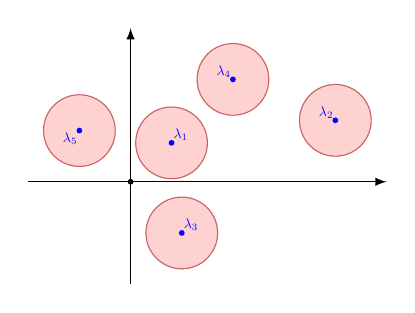
\begin{tikzpicture}[scale=1.3]
  \definecolor{mylightred}{RGB}{255,210,210}
  \definecolor{myred}{RGB}{200,100,100}
  \definecolor{mydarkred}{RGB}{140,40,40}
  \def\R{0.35}
  \def\ang{15}
  \coordinate (O)  at (0, 0);
  \coordinate (L1) at (0.4, 0.38);
  \coordinate (L2) at (2, 0.6);
  \coordinate (L3) at (0.5, -0.5);
  \coordinate (L4) at (1, 1);
  \coordinate (L5) at (-0.5, 0.5);
 
  \draw[-latex] (0, -1) -- (0, 1.5);
  \draw[-latex] (-1, 0) -- (2.5, 0);
  \fill[radius=0.8pt,black] (O) circle;
  \foreach \i in {1, ..., 5}{
     \draw[mylightred, fill] (L\i) circle (\R);
     \draw[myred] (L\i) circle (\R);
  }
  \fill[radius=0.8pt,blue]
    (L1) circle node[above right=-1pt,scale=0.5] {$\lambda_1$}
    (L2) circle node[above left =-1pt,scale=0.5] {$\lambda_2$}
    (L3) circle node[above right=-1pt,scale=0.5] {$\lambda_3$}
    (L4) circle node[above left =-1pt,scale=0.5] {$\lambda_4$}
    (L5) circle node[below left =-1pt,scale=0.5] {$\lambda_5$};
\end{tikzpicture}